\documentclass[11pt,a4paper]{article}

\usepackage[utf8]{inputenc}
\usepackage[T1]{fontenc}
\usepackage{lmodern}
\usepackage{amsmath,amssymb,amsfonts}
\usepackage{geometry}
\geometry{margin=1in}
\emergencystretch=3em
\usepackage{hyperref}
\hypersetup{colorlinks=true, linkcolor=blue, urlcolor=blue}
\usepackage{enumitem}
\usepackage{listings}
\usepackage{xcolor}
\usepackage{graphicx}
\graphicspath{{./}}
\usepackage{booktabs}
\usepackage{fancyhdr}
\usepackage{titlesec}

\definecolor{codebg}{gray}{0.96}
\definecolor{codeframe}{gray}{0.78}
\definecolor{codecomment}{rgb}{0.0,0.5,0.0}
\lstset{
  basicstyle=\ttfamily\small,
  breaklines=true,
  breakatwhitespace=false,
  postbreak=\mbox{\textcolor{codeframe}{$\hookrightarrow$}\space},
  frame=single,
  framerule=0.6pt,
  rulecolor=\color{codeframe},
  backgroundcolor=\color{codebg},
  keywordstyle=\color{blue},
  commentstyle=\color{codecomment},
  stringstyle=\color{red!70!black},
  showstringspaces=false,
  columns=flexible,
  xleftmargin=1.2em,
  xrightmargin=1.2em,
  aboveskip=1.1em,
  belowskip=1.1em
}

\titleformat{\paragraph}[hang]{\normalfont\normalsize\bfseries}{}{0pt}{}
\titlespacing*{\paragraph}{0pt}{1.7ex plus .6ex minus .2ex}{0.8ex}

\pagestyle{fancy}
\fancyhf{}
\fancyhead[L]{\textit{Tropical Monte Carlo v3}}
\fancyhead[R]{\textit{Reference Manual}}
\fancyfoot[C]{\thepage}

\title{\textbf{Tropical Monte Carlo v3} \\ \Large Comprehensive Reference Manual}
\author{}
\date{}

\begin{document}

\maketitle
\thispagestyle{empty}

\vfill
\begin{center}
\textit{A numerical integration pipeline for generalized Euler integrals \\
using tropical geometry and Monte Carlo sampling. \\[0.5em]
v3 = divergence/IBP engine (Tree A) $\cup$ lifting/complex engine (Tree B), \\
refactored into a single non-duplicated package with complex-lifting fixes baked in.}
\end{center}
\vfill

\newpage
\tableofcontents
\newpage

%=============================================================================
\section{Overview and Purpose}
%=============================================================================

The \textbf{Tropical Monte Carlo v3} project is a numerical integration pipeline for evaluating generalized Euler integrals of the form:
\begin{equation}\label{eq:main}
I = \int_{[0,\infty)^n} dx_1 \cdots dx_n \;\prod_{i} x_i^{A_i} \;\prod_{j} P_j(\mathbf{x})^{B_j}
\end{equation}
where:
\begin{itemize}
  \item $P_j(\mathbf{x})$ are polynomials in $\mathbf{x}$ with real or complex coefficients, possibly depending on kinematic parameters.
  \item $A_i \in \mathbb{C}$ are the monomial exponents, possibly depending on a dimensional regulator $\varepsilon$.
  \item $B_j \in \mathbb{C}$ are the polynomial exponents, possibly depending on $\varepsilon$.
\end{itemize}

v3 unifies the capabilities of two predecessor codebases:
\begin{itemize}
  \item \textbf{Tree A (\texttt{TROPICAL\_MONTE\_CARLO}):} divergence handling (tropical subtraction + IBP), batched VEGAS, factored C++ codegen. The base.
  \item \textbf{Tree B (\texttt{TROPICAL\_MONTE\_CARLOv2}):} auxiliary-variable lifting, complex exponents, \texttt{FlattenSector} refactoring, \texttt{SeedBase} runtime override. Grafted as Module 1b.
  \item \textbf{Bug-log complex-lifting branch (CALC2):} fixes for \texttt{SplitRealImag} mode (\texttt{MonoFactorLog}, complex \texttt{log P}), high-D fan K-scaling, high-D VEGAS sizing. Reconstructed from the bug logs as the genuinely new engineering of v3.
\end{itemize}

\paragraph{Exactness invariant (non-negotiable).} All tropical decomposition code is exact and symbolic. Floating-point arithmetic appears in exactly two places: (1)~the numerical integration of flattened sector integrands (MC/VEGAS), and (2)~independent numerical cross-checks (NIntegrate, CUBA). No decision inside the decomposition is made by evaluating a float.

\paragraph{Key innovation.} The code uses tropical geometry---the Newton polytope fan decomposition---to partition the integration domain into simplicial sectors. Within each sector, symbolic coordinate transformations and a ``flattening'' procedure render the integrand $\mathcal{O}(1)$ on $[0,1]^n$, making uniform Monte Carlo sampling highly efficient. A single C++ compilation handles thousands of kinematic points.

%=============================================================================
\section{Mathematical Background}
%=============================================================================

\subsection{The Problem}

Direct Monte Carlo on $[0,\infty)^n$ is impractical because the integrand has singular behavior near coordinate hyperplanes ($x_i \to 0$), different monomials dominate in different regions, and variance is enormous without importance sampling.

\subsection{Tropical Geometry Approach}

The tropical version of $P(\mathbf{x}) = \sum_m c_m \mathbf{x}^m$ replaces multiplication with addition and addition with $\min$:
\begin{equation}
\mathrm{trop}(P)(\mathbf{w}) = \min_m \{ m \cdot \mathbf{w} \} \qquad (\mathbf{w} \in \mathbb{R}^n)
\end{equation}

The \textbf{Newton polytope} $\mathrm{NP}(P)$ is the convex hull of the exponent vectors. Its \textbf{normal fan} partitions $\mathbb{R}^n$ into cones, one per vertex, each corresponding to a region where one monomial dominates. Refining into simplicial cones gives the fan used here.

\subsection{Why This Works}

In each cone, the dominant monomial is factored out symbolically (an exact algebraic identity). After a monomial change of variables aligned with the cone's rays, the remaining polynomial has no singular behavior. A further ``flattening'' substitution absorbs the monomial singularity $x^{A-1}$ into the measure, producing an $\mathcal{O}(1)$ integrand on $[0,1]^n$.

The fan depends only on the Newton polytope support (which monomials appear), not on coefficient values or the exponents $B_j$. For kinematic-dependent or extreme coefficients, compute the fan from a unit-coefficient proxy.

%=============================================================================
\section{File Structure}
%=============================================================================

\begin{lstlisting}
TROPICAL_MONTE_CARLO3/
|
|-- SUMMARY.txt               Concise API + limitations reference
|-- tropical_fan.wl           Tropical fan computation via Polymake
|                             (+ computeFanScaled for high-D lifting)
|-- tropical_eval.wl          Main evaluation package (merged, v3)
|                             M0: Primitives
|                             M1: ProcessSector, FlattenSector
|                             M1b: Lifting
|                             M2: Divergence subtraction
|                             M2b: IBP pole extraction
|                             M3: Unified C++ codegen
|                             M4: Unified driver
|                             M5: Validation
|
|-- EXAMPLES/                 Worked examples and tests
|-- TEST/                     43 named cross-checks + baselines/
|-- SANDBOX/                  Lifting development experiments
|-- CC/                       FIESTA cross-checks (optional dep.)
|-- INTERFILES/               Generated C++, binaries (gitignored)
|-- MANUAL/                   This manual
\end{lstlisting}

%=============================================================================
\section{Architecture: The 5-Feature Pipeline}
%=============================================================================

\subsection{Stage 1: Tropical Fan Decomposition (\texttt{tropical\_fan.wl})}
\begin{description}[style=nextline]
  \item[Input:] Newton polytope of $P_1 \cdots P_m$ (unit-coefficient proxy for kinematic or extreme coefficients)
  \item[Process:] Convex hull $\to$ normal fan $\to$ simplicial triangulation (via Polymake)
  \item[Output:] \texttt{\{dualVertices, simplexList\}}---integer ray generators plus simplicial cone $n$-tuples
  \item[v3 addition:] Private \texttt{computeFanScaled} retries on $K\!\cdot\!\mathrm{verts}$ with $K\in\{1,n+2,2n+4,6n+6\}$ (scale-invariant normal fan) to handle thin-simplex failures in dim~$\geq 4$.
\end{description}

\subsection{Stage 2: Symbolic Sector Processing}
\begin{description}[style=nextline]
  \item[Source:] Module 1---\texttt{ProcessSector}, \texttt{FlattenSector}
  \item[Process:] For each simplicial cone: (a) build ray matrix $M$, (b) monomial change of variables, (c) tropical factoring, (d) effective exponents, (e) convergence gate, (f) flattening
  \item[Output:] \texttt{SectorData} association per cone (see Section~\ref{sec:datastructs})
\end{description}

\texttt{FlattenSector} is factored out (from Tree B) and accepts an optional \texttt{eps} argument: the divergence predicate is evaluated at $\varepsilon\to 0$ when \texttt{eps} is present, enabling the lifted path to consume pre-flattening \texttt{ClearedPolys} before its own delta resolution.

\subsection{Stage 3a: Divergence Regulation}
\begin{description}[style=nextline]
  \item[Source:] Module 2 (subtraction) + Module 2b (IBP)
  \item[When:] Any sector has $\mathrm{Re}(a_{\mathrm{eff},k})|_{\varepsilon=0} \leq 0$
  \item[Limitation:] Single divergent variable per sector only. Nested divergences ($1/\varepsilon^{d\geq 2}$) refused cleanly (\texttt{\$Failed}). See Section~\ref{sec:limitations}.
\end{description}

Both methods are kept; IBP is the default (\texttt{Method\,-> Automatic} $\Rightarrow$ \texttt{"IBP"}); subtraction is the validating cross-check.

\subsection{Stage 3b: Auxiliary-Variable Lifting}
\begin{description}[style=nextline]
  \item[Source:] Module 1b---\texttt{DetectExtremeCoefficients}, \texttt{LiftCoefficients}, \texttt{ProcessSectorLifted}
  \item[When:] Polynomial coefficient $|C| \gg 1$ or $|C| \ll 1$ inflates MC variance
  \item[Composes with divergence (Case A):] a lifted sector may \emph{also} carry a single $1/\varepsilon$ pole. After the lifting $\delta$-resolution collapses the auxiliary dimension, a lifted sector is structurally an ordinary $n$-dimensional \texttt{SectorData} whose pole lives in one of the surviving effective exponents $\tilde a_j$---the object Stage~3a already consumes. \texttt{ProcessSectorLifted} is $\varepsilon$-aware and routes through the divergence machinery (Section~\ref{sec:liftdiv}). Refused cases: the divergent variable coupling to the lifted domain face (Case~B), \texttt{SplitRealImag}$\times$lift$\times$divergence, and complex-$B$ lifting.
\end{description}

\subsection{Stage 4: C++ Code Generation and Execution}
\begin{description}[style=nextline]
  \item[Source:] Module 3---\texttt{GenerateCpp}, \texttt{CompileCpp}, \texttt{detectCuba}
  \item[Process:] Translate Mathematica expressions $\to$ C++; generate integrand functions; generate \texttt{main()} (MC or VEGAS); compile; run; read results.
  \item[Samplers:] \texttt{"MC"} (default, plain uniform Monte Carlo) or \texttt{"VEGAS"} (CUBA-Vegas, opt-in; requires the CUBA library). Hard \texttt{\$Failed} if VEGAS requested but CUBA absent.
\end{description}

%=============================================================================
\section{Core Algorithms}\label{sec:algorithms}
%=============================================================================

\subsection{Sector Decomposition by Monomial Maps}

For a simplicial cone $\sigma$ with rays $\{\rho_1,\ldots,\rho_n\}$, define
\begin{equation}
M = -\mathrm{Transpose}[\rho_1,\ldots,\rho_n], \qquad
x_i = \prod_j y_j^{M_{ij}}, \quad \mathbf{y}\in(0,1]^n.
\end{equation}
The Jacobian and monomial prefactor combine to give raw exponents:
\begin{equation}
\mathrm{rawA}_j = \sum_i (A_i+1)\,M_{ij},
\end{equation}
and the sector integral reads $I_\sigma = |\det M|\int_{[0,1]^n}d^n y\;\prod_j y_j^{\mathrm{rawA}_j-1}\prod_k P_k(\mathbf{y}^M)^{B_k}$.

\subsection{Tropical Factoring (exact)}

For each polynomial $P_k$, define $d_{k,j} = \min_m\{e_{m,j}\}$ (min over all monomials) and factor:
\begin{equation}
P_k(\mathbf{y}) = \mathbf{y}^{d_k} \cdot Q_k(\mathbf{y}).
\end{equation}
This is an exact algebraic identity for any coefficient values. The cleared polynomial $Q_k$ has all non-negative exponents and contains a constant term (the vertex-dual dominant monomial), giving $Q_k(\mathbf{y})\geq c_{\mathrm{dom}}>0$ on $[0,1]^n$.

\subsection{Effective Exponents and Convergence Gate}

\begin{equation}\label{eq:aeff}
a_{\mathrm{eff},j} = \mathrm{rawA}_j + \sum_k B_k\,d_{k,j} \in \mathbb{C}.
\end{equation}

A sector is convergent if $\mathrm{Re}(a_{\mathrm{eff},j})>0$ for all $j$ (evaluated at $\varepsilon=0$ when a regulator is present). The imaginary parts of $A_i$ and $B_j$ contribute to $a_{\mathrm{eff}}$ but do not affect convergence.

\subsection{Flattening}

\begin{equation}
y_j = (y'_j)^{1/a_j} \implies y_j^{a_j-1}\,dy_j = \frac{1}{a_j}\,dy'_j.
\end{equation}

The $y^{a-1}$ factor is completely absorbed. The sector integral becomes:
\begin{equation}\label{eq:master}
\boxed{I = \sum_\sigma \frac{|\det M_\sigma|}{\prod_j a_j^\sigma}
\int_{[0,1]^n} d^n y'\;\prod_k Q_k^\sigma\!\bigl(\mathbf{y}'^{1/a^\sigma}\bigr)^{B_k}}
\end{equation}

For complex $a_j$, this is the analytic continuation; geometrically, $\mathrm{Im}(a_j)\neq 0$ rotates the integration contour onto a logarithmic spiral and additionally suppresses MC variance. See Figure~\ref{fig:complex_flatten_spiral}.

\begin{figure}[ht]
\centering
% complex_flatten_spiral.pdf from Tree B MANUAL/ (TROPICAL_MONTE_CARLOv2/MANUAL/)
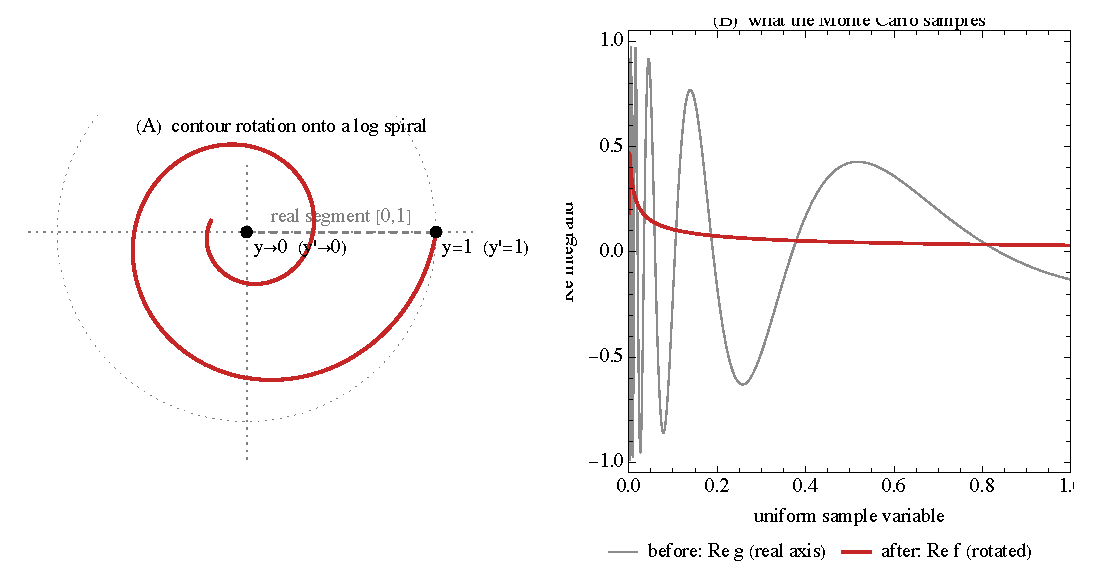
\includegraphics[width=0.6\textwidth]{complex_flatten_spiral}
\caption{Complex flattening contour rotation. When $a_j$ has a nonzero imaginary part, the substitution $y_j=(y'_j)^{1/a_j}$ rotates the sector's integration contour onto a logarithmic spiral in the complex plane. This suppresses the oscillatory contributions from $B_k\in\mathbb{C}$ and can dramatically reduce Monte Carlo variance. Reproduced from Tree B \texttt{MANUAL/complex\_flatten\_spiral.pdf}.}
\label{fig:complex_flatten_spiral}
\end{figure}

\subsection{Divergence Regulation: Tropical Subtraction (Module 2)}

When $a_k(\varepsilon) = c_k\varepsilon + \mathcal{O}(\varepsilon^2)$ with $c_k>0$:
\begin{equation}
I_{\mathrm{sector}} = \frac{G_0}{c_k\varepsilon} + \frac{G_1}{c_k} + R + \mathcal{O}(\varepsilon)
\end{equation}
where:
\begin{description}
  \item[$G_0$:] $(n{-}1)$-dim integral with $y_k=0$ (pole coefficient).
  \item[$G_1$:] $G_0$ integrand times log-insertion sum $\sum_i\frac{a_i^{(1)}}{a_i^{(0)}}\log y'_i + \sum_j B_j^{(1)}\log Q_j|_{y_k=0}$.
  \item[$R$:] Remainder $\int[F_{\mathrm{full}}-F_{\mathrm{simple}}]\cdot y_k^{a_{k}^{(0)}-1}\,d\mathbf{y}$ (convergent at $\varepsilon=0$).
\end{description}
The analytic pole $1/c_k$ is computed symbolically; $G_0$, $G_1$, $R$ are evaluated numerically.

\subsection{Divergence Regulation: IBP (Module 2b, default)}

Integration by parts on $[0,1]$ for the divergent variable $y_k$:
\begin{equation}
\int_0^1 y_k^{a_k-1}f\,dy_k = \frac{1}{a_k}\Bigl[f\big|_{y_k=1} - \int_0^1 y_k^{a_k}\partial_{y_k}f\,dy_k\Bigr]
\end{equation}
$\partial_{y_k}\prod_j Q_j^{B_j}$ decomposes into monomial terms, each with shifted exponents $\alpha_{t,k}=a_k+e_{m,k}\geq 1$ at $\varepsilon=0$ (convergent). The analytic pole structure:
\begin{align}
\text{Pole:}\quad & \frac{B^{(0)} - S_0}{c_k\varepsilon} \\
\text{Finite:}\quad & \frac{(B^{(1)}-S_1) - r_k(B^{(0)}-S_0)}{c_k}
\end{align}
where $S_0=\sum_t\mathrm{coeff}_t^{(0)}I_{t,0}$, $r_k=a_k^{(2)}/c_k$. IBP and subtraction agree on (pole, finite) to $\lesssim 10^{-3}$ (cross-check \#4); this agreement is one of the strongest correctness signals in v3.

\subsection{Auxiliary-Variable Lifting (Module 1b)}\label{sec:lifting}

Replace the extreme coefficient $C$ in monomial $C\mathbf{x}^\alpha$ by $z^k\mathbf{x}^\alpha$, with anchor $z_0=|C|^{1/k}$ (kept exact in Mathematica) and residual $c=C/z_0^k$ (the $\mathcal{O}(1)$ phase or sign). Insert $\int dz\,\delta(z-z_0)$. The $(n{+}1)$-dimensional lifted integrand is decomposed on the fan of the lifted polynomial; the delta constraint is resolved per sector by a pivot substitution.

\subsubsection{Anchor Selection ($k^*$ rule)}\label{sec:anchor}

The anchor $z_0 = |C|^{1/k}$ and the integer $k$ are locked together: $k$ must be a positive integer (it is the $z$-exponent in the lifted monomial and a lattice coordinate of the lifted Newton polytope), so choosing $k$ determines $z_0$ completely. The optimal stopping point is self-consistency with the detector: the package already flags a coefficient as extreme when it leaves the band $[1/\tau,\tau]$ (threshold $\tau$, default $10^3$), so pick the \emph{smallest} $k$ that brings the anchor back into the band:
\begin{equation}\label{eq:kstar}
  k^{*} = \max\!\Bigl(1,\;\Bigl\lceil\tfrac{|\log|C||}{\log\tau}\Bigr\rceil\Bigr)
  \;\xrightarrow{\;\tau=10^3\;}\; \max\!\Bigl(1,\;\bigl\lceil\tfrac{\log_{10}|C|}{3}\bigr\rceil\Bigr).
\end{equation}
Going past $k^{*}$ buys only sub-threshold residual shrinkage while paying geometry cost (inflated $|\det M|$, shrunken integrability margins, more \texttt{EmptyDomain} sectors). The same formula covers both large and small coefficients (it uses $|\log|C||$). Worked cases from the v3 benchmarks:

\begin{center}\small
\begin{tabular}{lcccl}
\toprule
Case & $|C|$ & $k^{*}$ & $z_0=|C|^{1/k^{*}}$ & hand-picked $k$ \\
\midrule
Case A ($10^6 x_1^2$) & $10^6$ & $2$ & $10^3$ & $2$ \\
Case B primary ($10^4 x_1^2$) & $10^4$ & $2$ & $10^2$ & $2$ \\
Example 20 ($10^{-4} x_1^2$) & $10^{-4}$ & $2$ & $10^{-2}$ & $2$ \\
\bottomrule
\end{tabular}
\end{center}

\paragraph{Decision order.} (1)~Geometry gate first: require a surviving sector with \texttt{HasConstantTerm=True} and all $\mathrm{Re}[\tilde{a}]>0$; if no such sector exists for any $k$, \textbf{do not lift}. (2)~Smallest $k$ with $z_0\in[1/\tau,\tau]$ (i.e.\ $k^{*}$). (3)~Simpler geometry (lower $|\det M|$, fewer empty sectors). The full procedure, including the multi-rule multi-coefficient case, is in the file \texttt{AUXT/anchor\_selection\_procedure.md} under \texttt{OLD\_CODE/TROPICAL\_MONTE\_CARLO2/TROPICAL\_MONTE\_CARLOv2/}.

\subsubsection{Pivot Selection and Delta Elimination}

For a simplicial cone with $(n{+}1)$-dimensional sector data, let $m=(m_1,\ldots,m_{n+1})$ be the $z$-row of the ray matrix. Select a pivot $p$ with $m_p\neq 0$. The delta constraint gives:
\begin{equation}
y_p^* = z_0^{1/m_p}\prod_{j\neq p}y_j^{-m_j/m_p}
\end{equation}
Substituting this in the cleared polynomial, re-clearing (Step 2 repeated), and absorbing the delta Jacobian produces an $n$-dimensional sector with effective exponents:
\begin{equation}
\tilde{a}_j = a_j - a_p\frac{m_j}{m_p} + \sum_k B_k\tilde{d}_{k,j}, \qquad
\text{prefactorBase} = \frac{|\det M|}{|m_p|}z_0^{a_p/m_p-1}.
\end{equation}

\paragraph{Pivot ranking (constant-term preservation first):}
\begin{enumerate}
  \item \texttt{HasConstantTerm = True} after re-clearing. \emph{First because sectors without a constant term can have infinite true variance (L5 risk, Section~\ref{sec:limitations}).}
  \item $|m_p|=1$ (unit pivot exponent).
  \item $\max\min_j\mathrm{Re}[\tilde{a}_j]$ (best integrability margin).
\end{enumerate}

\paragraph{Domain constraint.} The lifted sector only contributes where $y_p^*\in(0,1]$, i.e.\ $\log y_p^*\leq 0$. Sign analysis classifies sectors as: always feasible (no indicator), never feasible (\texttt{EmptyDomain}, returned and dropped), or mixed. The domain-constraint indicator in the flattened variables $y'_j=(y_j)^{\tilde{a}_j}$ is:
\begin{equation}
\log y_p^* = \frac{1}{m_p}\Bigl(\log z_0 - \sum_{j\neq p}\frac{m_j}{\tilde{a}_j}\log y'_j\Bigr) \leq 0,
\end{equation}
compiled into the C++ integrand (returns 0 outside the feasible region).

\subsubsection{\texttt{HasConstantTerm = False}: the L5 Caveat}

When the re-cleared polynomial $\tilde{Q}$ lacks a constant term, the lifted integrand may not be in $L^2$ on $[0,1]^n$. The sample-based standard error understates the true error; the MC estimate can significantly deviate from the true value. Always cross-check against an independent reference (NIntegrate, CUBA Cuhre) rather than trusting the MC error bar for \texttt{HasConstantTerm=False} sectors.

\subsubsection{Lifting a Divergent Integral (Case A)}\label{sec:liftdiv}

Lifting and a simple $1/\varepsilon$ pole compose. The two features act on different objects: lifting acts on a polynomial \emph{coefficient} (a $+1$-dimensional $\delta$-constraint), while divergence acts on a monomial \emph{exponent} $a_k(\varepsilon)\to 0$ (a $1/\varepsilon$ endpoint pole). After the $\delta$-resolution collapses the auxiliary dimension, the pole---if any---necessarily sits in one of the $n$ post-$\delta$ effective exponents $\tilde a_j$, exactly the object the IBP/subtraction machinery consumes.

\paragraph{$\varepsilon$-aware classification.} \texttt{ProcessSectorLifted[\ldots,\,"Eps"->eps]} classifies each $\tilde a_j$ at $\varepsilon\to 0$ \emph{exactly} (\texttt{PossibleZeroQ[Im]} and \texttt{Re[\ldots]>0}, never a tolerance): \texttt{"complex"} ($\to$\,\texttt{liftcomplex}), \texttt{"convergent"} ($\mathrm{Re}>0$), or \texttt{"divergent"} ($\mathrm{Re}\leq 0$, regulator present). A pivot is admissible iff no direction is complex and \emph{at most one} is divergent (with $c_k=\partial_\varepsilon\tilde a_k|_0\neq 0$). With \texttt{"Eps"->None} the classification reduces exactly to the pre-$\varepsilon$ realness test, so convergent lifting is byte-identical.

\paragraph{Prefactor $\varepsilon$-dependence.} A divergent lifted \texttt{SectorData} carries \texttt{"PrefactorBase"} $=(|\det M|/|m_p|)\,z_0^{a_p/m_p-1}$, which itself carries $\varepsilon$ through $a_p(\varepsilon)$. The divergence routines use \texttt{PrefactorBase}$|_{\varepsilon=0}$ in the integrand and the IBP Laurent assembly adds the missing finite term $(\partial_\varepsilon\log\text{PrefactorBase})|_0\cdot(\text{pole})$, stored as \texttt{"DLogPrefactor"} ($=0$ for unlifted sectors).

\paragraph{Case A vs Case B.} The lifted domain indicator has coefficients $\mathrm{ic}_j=m_{\text{other},j}/\tilde a_j$. \emph{Case A} (supported): the divergent slot decouples ($\texttt{DomainConstraint}\,\texttt{===}\,\texttt{None}$ or $\mathrm{ic}_k=0$, i.e.\ $m_{\text{other},k}=0$); the indicator commutes with the $y_k$ IBP/subtraction and rides along on the other coordinates. \emph{Case B} (refused, \texttt{liftdivdomain}): $\mathrm{ic}_k\neq 0$ for \emph{every} admissible pivot. The pivot ranking adds a \emph{Case-A-first} key so a decoupled pivot wins whenever one exists; Case B is refused only when none does (rare---no trigger found across a diverse $n=2,3,4$ battery).

\paragraph{Two routes.} Both Stage-3a routes resolve the lifted Laurent (cross-checks 41-C and 45, $n=2,3,4$, non-trivial polynomials). \texttt{LaurentFromSubtraction} (pin $\varepsilon$, sum the full decomposition, fit) is the \emph{robust universal} route---it does not rely on per-sector pole classification, so it is correct even when non-trivial polynomials produce \texttt{HasConstantTerm=False} sectors. The per-sector \texttt{Method->"IBP"} route is exact only when every sector is \texttt{HasConstantTerm}-clean; otherwise a convergent sector can carry a polynomial-zero pole ($\tilde Q_j\to 0$, $B_j<0$) that the $\tilde a$-classification misses and the IBP pole undercounts (a pre-existing sector-decomposition limitation, not specific to lifting). Use the Subtraction route there.

\subsection{Complex Exponents in Codegen}\label{sec:complexcodegen}

The default complex-exponent path (\texttt{ComplexExponentMode -> "Direct"}) evaluates:
\begin{equation}
\text{\texttt{result *= std::exp(B\_j * std::log(P\_j));}} \quad (\text{complex \texttt{log}})
\end{equation}
This is always correct. For polynomial exponents $B_j\in\mathbb{C}$ and polynomials with complex coefficients ($\arg P\neq 0$), the complex \texttt{log} is essential.

The opt-in \texttt{"SplitRealImag"} VEGAS-variance mode uses the split identity:
\begin{equation}
\prod_j P_j^{B_j} = \prod_j P_j^{\mathrm{Re}(B_j)}\cdot\exp\!\Bigl(i\sum_j \mathrm{Im}(B_j)\log P_j\Bigr)
\end{equation}
\textbf{Two fixes are required} before this mode is correct:

\paragraph{Fix A (BUG 1, \texttt{TMCv2\_BUG\_LOG}).} Use the complex \texttt{log}. The oscillatory phase $\exp(i\,\mathrm{Im}(B)\log P)$ splits as $\exp(-\mathrm{Im}(B)\arg P)\cdot\exp(i\,\mathrm{Im}(B)\log|P|)$; using \texttt{std::log(std::abs(P))} silently drops the factor $\exp(-\mathrm{Im}(B)\arg P)$, which equals 1 only for real-positive $P$. With complex coefficients $\arg P\neq 0$, so this bug is invisible in all real-coefficient tests but wrong in general.

\paragraph{Fix B (L3, \texttt{lift\_error\_log}).} Restore the tropical monomial factor. Tropical factoring removed the monomial $\mathbf{y}^{d_k}$; the oscillatory phase must add back:
\begin{equation}
\sum_k\mathrm{Im}(B_k)\bigl(\mathrm{Const}_k + \sum_i\mathrm{Coeffs}_{k,i}\log y'_i\bigr),
\end{equation}
where for unlifted sectors $\mathrm{Const}=0$, $\mathrm{Coeffs}_i=d_{k,i}/a_{\mathrm{eff},i}$; for lifted sectors the residual exponents include contributions from the pivot substitution. Stored as \texttt{SectorData["MonoFactorLog"] = \{Const, Coeffs\}}.

\paragraph{\texttt{SplitRealImag} caveat.} For very large $\mathrm{Im}(B)$, VEGAS importance sampling built on $\mathrm{Re}(B)$ can inflate variance. Always compare \texttt{SplitRealImag} against \texttt{Direct} and an independent reference before trusting \texttt{SplitRealImag} results. The default \texttt{"Direct"} mode is always safe.

\subsection{High-Dimensional VEGAS Sizing (\texttt{resolveVegasSizing})}\label{sec:vegassizing}

VEGAS defaults (\texttt{NStart=1000, NIncrease=500, NBatch=1000}) are tuned for $n\leq 4$. For sector dimension $d\geq 6$ they return confidently wrong values with deceptively tight error bars (measured: 8D unlifted 1.2\% off at $7\sigma$; lifted $\sim$45\% off). The fix: resolve \texttt{Automatic} via $\texttt{NStart}\approx\text{base}\cdot 3^{d-4}$ for $d\geq 5$; fire \texttt{TropicalEval::vegasbudget} when \texttt{NSamples}$<20\cdot$\texttt{NStart}. In high dimensions, always cross-check against an independent reference rather than trusting the VEGAS error bar.

%=============================================================================
\section{Core File Reference}
%=============================================================================

\subsection{\texttt{tropical\_fan.wl}}\label{sec:fan-api}

\begin{description}
  \item[\texttt{PolytopeVertices[integrand, vars]}] Extracts Newton polytope lattice points from the integrand.
  \item[\texttt{ComputeDecomposition[vertices]}] Returns \texttt{\{dualVertices, simplexList\}}. Internally calls the private \texttt{computeFanScaled} for automatic K-scaling retry on degenerate thin-simplex cases.
  \item[\texttt{computeFanScaled[vertices]}] \emph{(private)} The K-scaling fan helper in \texttt{tropical\_fan.wl}: retries the normal-fan computation on $K\!\cdot\!\mathrm{verts}$ with $K\in\{1,n+2,2n+4,6n+6\}$ (scale-invariant normal fan) to recover from thin-simplex failures in dim~$\geq 4$. Used both by \texttt{ComputeDecomposition} and by \texttt{EvaluateTropicalMCLifted}'s automatic \texttt{"FanData"} path (Section~\ref{sec:lifted-api}).
  \item[\texttt{ComputeDecompositiony[vertices]}] Variant intersecting with the positive orthant.
  \item[\texttt{convexHullVertices[points]}] Calls Polymake to compute the convex hull.
  \item[\texttt{translateToOriginInteger[vertices]}] Shifts polytope so the origin is an interior lattice point.
  \item[\texttt{\$TropicalFanPolymakePath}] Override Polymake auto-detection before loading.
  \item[\texttt{\$SkipPolymakeLoad}] Set to \texttt{True} before loading to skip \texttt{tropical\_fan.wl} (for cluster nodes without Polymake; supply \texttt{fanData} explicitly).
\end{description}

The fan properties required by the evaluation algorithm: (1)~simpliciality ($\det\neq 0$; violations caught by \texttt{degenerate}/\texttt{notsimplicial}), (2)~completeness ($\bigcup_\sigma=\mathbb{R}^n$), (3)~essential disjointness, (4)~vertex duality (one monomial of each $P_k$ attains the tropical minimum throughout the cone---guarantees the constant term in $Q_k$).

\subsection{\texttt{tropical\_eval.wl} --- Module 1: \texttt{ProcessSector} and \texttt{FlattenSector}}

\begin{lstlisting}
ProcessSector[integrandSpec, dualVertices, simplex, coneIndex]
FlattenSector[clearedPolys, effectiveAVals, prefactorBase, eps:None]
\end{lstlisting}

\texttt{ProcessSector} executes Steps 1--3 (monomial map, tropical factoring, effective exponents) and calls \texttt{FlattenSector} for Step 4 (flattening). When \texttt{eps} is passed, the divergence predicate evaluates effective exponents at $\varepsilon\to 0$ via:
\begin{lstlisting}[language=Mathematica]
a0 = If[eps =!= None, effectiveAVals /. eps -> 0, effectiveAVals];
isDivergent = Or @@ (TrueQ[Re[#] <= 0] & /@ a0);
\end{lstlisting}

The \texttt{IsDivergent -> True} pre-flattening early-return branch of \texttt{ProcessSector} is preserved: the lifted path consumes \texttt{ClearedPolys}/\texttt{NewExponents} from it, because $(n{+}1)$-dim pre-delta sectors are routinely flagged divergent even when the delta-constrained integral is finite.

\paragraph{\texttt{CheckFlatteningMagnitude[sectorData, nSamples]}.} Evaluates the flattened integrand at random points in $[0,1]^n$, reporting min/max/mean magnitude and warning when $\max>10^3$ or $\min<10^{-6}$ (a heavy-tail indicator). For lifted sectors with a \texttt{DomainConstraint}, draws feasible points by rejection sampling and additionally returns \texttt{"FeasibleFraction"}.

\subsection{\texttt{tropical\_eval.wl} --- Module 1b: Lifting}

\begin{description}
  \item[\texttt{DetectExtremeCoefficients[spec, threshold:1000, opts]}] Returns a list of associations \texttt{\{<|"PolyIndex","ExponentVector","Coefficient","Magnitude","SuggestedK"|>\}} for every monomial with $|C|<1/\tau$ or $|C|>\tau$. \texttt{SuggestedK} uses the $k^*$ rule (Section~\ref{sec:anchor}). Symbolic coefficients skipped.

  \item[\texttt{LiftCoefficients[spec, liftRules]}] Applies lifting: each rule is \texttt{<|"PolyIndex"->j,"ExponentVector"->$\alpha$,"k"->k|>}. Returns \texttt{<|"LiftedSpec"->...,"LiftData"->...|>}. Performs the round-trip identity check ($z\to z_0$ recovers the original polynomial exactly); fires \texttt{liftidentity} on failure.

  \item[\texttt{ProcessSectorLifted[liftedSpec, dualVerts, simplex, coneIndex, liftData]}] Runs \texttt{ProcessSector} in dimension $n{+}1$, then resolves the delta constraint (pivot selection, substitution, re-clearing, domain analysis). Returns \texttt{SectorData} extended with lifted keys. Error paths: \texttt{liftnopivot}, \texttt{liftcomplex}, \texttt{liftdivergent}.

  \item[\texttt{ValidateLiftedDecomposition[origSpec, liftedSpec, liftedFan, liftData, kin, pg]}] Cross-checks the lifted sector sum against direct \texttt{NIntegrate} of the original integral. Returns \texttt{DirectResult}, \texttt{SectorSum}, \texttt{RelativeError}, \texttt{SectorResults}, \texttt{DroppedSectors}.
\end{description}

\subsection{\texttt{tropical\_eval.wl} --- Module 2: Tropical Subtraction}

\begin{description}
  \item[\texttt{IdentifyDivergences[sectorData, eps]}] Expands effective exponents in $\varepsilon$, finds variables with $\mathrm{Re}(a_k(0))\leq 0$. Returns divergent variable index, $c_k$, $a^{(0)}$, $a^{(1)}$.
  \item[\texttt{ProcessDivergentSector[sectorData, integrandSpec]}] Constructs $G_0$, $G_1$, Remainder. Returns \texttt{DivergentSectorData}.
  \item[\texttt{ValidateSubtraction[divSD, sd, spec, kin, eps]}] Cross-checks $G_0/(c_k\varepsilon)+G_1/c_k+R$ against direct \texttt{NIntegrate} at finite $\varepsilon$.
\end{description}

\subsection{\texttt{tropical\_eval.wl} --- Module 2b: IBP (default method)}

\begin{description}
  \item[\texttt{IBPReduceSector[sectorData, eps]}] Symbolic IBP decomposition: identifies all divergent variables and iteratively applies IBP to produce convergent terms. Returns \texttt{IBPPrefactors}, \texttt{Terms}, \texttt{DivergentVariables}, \texttt{NTerms}.
  \item[\texttt{IBPProcessSector[sectorData, integrandSpec]}] Full pipeline: reduction + $\varepsilon$-expansion + per-term flattening + boundary construction. Returns \texttt{IBPSectorData}.
  \item[\texttt{IBPCheckBoundary[sectorData, integrandSpec, nPoints]}] Verifies IBP boundary terms numerically.
  \item[\texttt{ValidateIBP[ibpSD, sd, spec, kin, eps]}] Cross-checks IBP formula against \texttt{NIntegrate} at finite $\varepsilon$. Returns \texttt{RelativeError}.
\end{description}

\subsection{\texttt{tropical\_eval.wl} --- Module 3: Unified C++ Codegen}

\paragraph{\texttt{MmaToC[expr, paramMap]}.} Recursive converter Mathematica $\to$ C++:
\begin{center}
\begin{tabular}{ll}
\toprule
\textbf{Mathematica} & \textbf{C++} \\
\midrule
Integer $n$ & \texttt{n.0} \\
Rational $p/q$ & \texttt{(p.0/q.0)} \\
\texttt{Complex[a,b]} & \texttt{cx(a, b)} \\
\texttt{Power[x, -1]} & \texttt{(1.0/x)} \\
\texttt{Power[x, 1/2]}, \texttt{Power[x,-1/2]} & \texttt{std::sqrt(x)}, \texttt{(1.0/std::sqrt(x))} \\
\texttt{Power[E, z]}, \texttt{Exp[z]} & \texttt{std::exp(z)} \\
\texttt{Power[x, e]} & \texttt{std::pow(x, e)} \\
\texttt{Log[x]} & \texttt{std::log(x)} \\
\texttt{Re[z]}, \texttt{Im[z]} & \texttt{(z).real()}, \texttt{(z).imag()} \\
Kinematic symbol & \texttt{params[i]} \\
\bottomrule
\end{tabular}
\end{center}

The \texttt{badcpp} gate: after generation, if any emitted code contains unconverted Mathematica heads or \texttt{ComplexInfinity}/\texttt{Indeterminate}, \texttt{GenerateCpp} returns \texttt{\$Failed} (\texttt{TropicalEval::badcpp}) instead of writing uncompilable C++.

Polynomial evaluation uses the \textbf{log-exp trick}:
\begin{equation}
c\cdot y_1^{\alpha_1}\cdots y_n^{\alpha_n} = c\cdot\exp(\alpha_1\log y_1+\cdots+\alpha_n\log y_n),
\end{equation}
which is branch-cut free for $y_i\in(0,1]$ and works for complex $\alpha_i$.

\paragraph{\texttt{GenerateCpp[convSectors, divSectors, spec, outputFile, opts]}.}

Generates a complete, self-contained C++ source file with integrand functions of all types:
\begin{description}
  \item[\texttt{integrand\_conv\_N}:] Convergent sector. For lifted sectors, includes the domain-constraint indicator (returns 0 outside the feasible region).
  \item[\texttt{integrand\_g0\_N}:] $G_0$ integral ($(n-1)$-dim, $y_k=0$ simplified polys).
  \item[\texttt{integrand\_g1\_N}:] $G_1$ integral ($G_0\times$ log-insertion sum).
  \item[\texttt{integrand\_rem\_N}:] Remainder ($\mathrm{prefactor}\times y_k^{a_k^{(0)}-1}\times[F_\mathrm{full}-F_\mathrm{simple}]$).
  \item[IBP types:] Boundary and term integrands, parametrized by the integrand-type tag.
\end{description}

The \texttt{main()} reads kinematic points from an input file, loops over points (OpenMP-parallelized for MC; serial for VEGAS to avoid CUBA thread-safety issues), draws samples, accumulates mean and variance with Welford's online algorithm, and writes one line per kinematic point: \texttt{re~~im~~err\_re~~err\_im}.

\paragraph{Sampler options (Table~\ref{tab:sampler}).}
\begin{table}[htbp]
\centering
\begin{tabular}{lll}
\toprule
\textbf{Option} & \textbf{Default} & \textbf{Description} \\
\midrule
\texttt{"Integrator"} & \texttt{"MC"} & \texttt{"MC"} (plain uniform) or \texttt{"VEGAS"} (CUBA-Vegas) \\
\texttt{"Batch"} & \texttt{False} & VEGAS only: share one LDS sample set across kinematic chunk \\
\texttt{"VegasEpsRel"} & \texttt{Automatic} & Vegas relative tolerance (tiny default makes maxeval binding) \\
\texttt{"VegasEpsAbs"} & \texttt{Automatic} & Vegas absolute tolerance \\
\texttt{"VegasSeed"} & \texttt{0} & CUBA seed; 0 = Sobol (deterministic) \\
\texttt{"VegasNStart"} & \texttt{Automatic} & Resolved by \texttt{resolveVegasSizing} \\
\texttt{"VegasNIncrease"} & \texttt{Automatic} & Resolved by \texttt{resolveVegasSizing} \\
\texttt{"VegasNBatch"} & \texttt{Automatic} & Resolved by \texttt{resolveVegasSizing} \\
\texttt{"VegasMinEval"} & \texttt{0} & CUBA mineval \\
\texttt{"CubaMaxComp"} & \texttt{512} & Batch-mode \texttt{ncomp} ceiling \\
\texttt{"NSamples"} & \texttt{10\textasciicircum{}6} & samples/sector for MC; maxeval/sector for VEGAS \\
\texttt{"SeedBase"} & \texttt{42} & Per-kp RNG seed base; also runtime \texttt{argv[5]} override \\
\bottomrule
\end{tabular}
\caption{Sampler options on \texttt{GenerateCpp}, \texttt{CompileCpp}, and \texttt{EvaluateTropicalMC}.}
\label{tab:sampler}
\end{table}

\paragraph{Batch mode (\texttt{"Batch" -> True}).} VEGAS only, convergent/lifted-convergent path only. Shares one low-discrepancy sample set across a chunk of kinematic points (up to \texttt{CubaMaxComp}/2 points per chunk for complex integrands; hard ceiling to avoid CUBA segfault). Divergent/IBP path falls back to per-kp VEGAS. Typically 30--60$\times$ wall-clock speedup on large scans.

\paragraph{CUBA detection and threading.} \texttt{detectCuba[]} is memoized and detects the \texttt{TROPICAL\_REQUIRES\_CUBA} sentinel in the generated source. If VEGAS is requested but CUBA is absent, compilation fails fast with an actionable message (\texttt{TropicalEval::nocuba}); no silent MC fallback. CUBA is not thread-safe across concurrent calls; Vegas mains loop serially with \texttt{cubacores(0,0)}. To use many cores on a large scan, shard the kinematic file across processes or use batch mode.

\subsection{\texttt{tropical\_eval.wl} --- Module 4: Unified Driver}

\begin{lstlisting}[language=Mathematica]
EvaluateTropicalMC[integrandSpec, fanData, kinematicPoints, opts...]
\end{lstlisting}

Routes on \texttt{"Method"} ($\in$ \texttt{\{Automatic, "None", "IBP", "Subtraction"\}}) and \texttt{"LiftData"} ($\in$ \texttt{\{None, <association from \texttt{LiftCoefficients}>\}}). The 10-step skeleton is shared: workdir $\to$ fan unpack $\to$ per-sector processing $\to$ optional Validate $\to$ codegen $\to$ compile $\to$ run $\to$ readback $\to$ assemble $\to$ error summary.

Thin wrappers for API continuity:
\begin{description}
  \item[\texttt{EvaluateTropicalMCLifted[spec, kin, opts]}] Auto-detects/applies lifting and routes through the unified driver via the \texttt{"LiftData"} option (see Section~\ref{sec:lifted-api}). This is the typical user-facing entry point for lifting; the bare \texttt{"LiftData"} option on \texttt{EvaluateTropicalMC} is the advanced/low-level path.
  \item[\texttt{LaurentFromSubtraction[spec, fan, kin, opts]}] Forces \texttt{"Method" -> "Subtraction"} and returns the Laurent expansion as \texttt{<|{-1} -> pole, 0 -> finite|>}.
  \item[\texttt{EvaluateTropicalMCIBP[spec, fan, kin, opts]}] Superseded by \texttt{EvaluateTropicalMC[..., "Method" -> "IBP"]} (which routes to the same private driver); kept for backward compatibility.
\end{description}

\paragraph{Full option list.}
\begin{center}
\begin{tabular}{lll}
\toprule
\textbf{Option} & \textbf{Default} & \textbf{Description} \\
\midrule
\texttt{"Method"} & \texttt{Automatic} & \texttt{"None"|\,"IBP"|\,"Subtraction"}; Auto $\Rightarrow$ IBP if divergent \\
\texttt{"LiftData"} & \texttt{None} & Association from \texttt{LiftCoefficients[]} or \texttt{None}; advanced/low-level path (typical users call \texttt{EvaluateTropicalMCLifted}); may be combined with \texttt{Method->"IBP"/"Subtraction"} for a lifted$+$divergent sector (Case~A, Section~\ref{sec:liftdiv}) \\
\texttt{"Integrator"} & \texttt{"MC"} & \texttt{"MC"} or \texttt{"VEGAS"} \\
\texttt{"EpsilonValue"} & \texttt{None} & Substitute $\varepsilon\to\text{value}$ (all sectors become convergent) \\
\texttt{"ComplexExponentMode"} & \texttt{Automatic} & \texttt{"Direct"} or \texttt{"SplitRealImag"} (see Section~\ref{sec:complexcodegen}) \\
\texttt{"NSamples"} & \texttt{10\textasciicircum{}6} & Samples per sector \\
\texttt{"NThreads"} & \texttt{Automatic} & OpenMP threads (\texttt{\$ProcessorCount}) \\
\texttt{"SeedBase"} & \texttt{42} & RNG seed base \\
\texttt{"RunChecks"} & \texttt{True} & Symbolic Validate* gating before the run \\
\texttt{"PrecisionGoal"} & \texttt{3} & Precision goal for validation integrals \\
\texttt{"Verbose"} & \texttt{True} & Progress output \\
\texttt{"WorkingDirectory"} & \texttt{Automatic} & Where generated files go (\texttt{INTERFILES/}) \\
\multicolumn{3}{l}{Plus all sampler options from Table~\ref{tab:sampler}.} \\
\bottomrule
\end{tabular}
\end{center}

\paragraph{\texttt{EvaluateTropicalMCLifted} signature and options.}\label{sec:lifted-api}
\begin{lstlisting}[language=Mathematica]
EvaluateTropicalMCLifted[integrandSpec, kinematicPoints, opts...]
\end{lstlisting}
The thin lifting wrapper: it detects/applies lifting (calling \texttt{DetectExtremeCoefficients} then \texttt{LiftCoefficients} internally), builds the $(n{+}1)$-dimensional lifted fan, and routes through \texttt{EvaluateTropicalMC} with the resulting \texttt{"LiftData"}. With no extreme coefficients it falls back to plain \texttt{EvaluateTropicalMC} on the original spec. Its five own options (it also forwards all \texttt{EvaluateTropicalMC} options):
\begin{center}
\begin{tabular}{lll}
\toprule
\textbf{Option} & \textbf{Default} & \textbf{Description} \\
\midrule
\texttt{"LiftRules"} & \texttt{Automatic} & Auto-detect extreme coefficients via \texttt{DetectExtremeCoefficients}, or supply explicit rules \\
\texttt{"Threshold"} & \texttt{1000} & Extreme-coefficient magnitude threshold passed to \texttt{DetectExtremeCoefficients} \\
\texttt{"AnchorRule"} & \texttt{"kStar"} & Anchor $z_0=|C|^{1/k}$ selection (\texttt{"kStar"} default; \texttt{"Unit"} = legacy) \\
\texttt{"BandEdgeGuard"} & \texttt{False} & Band-edge guard in extreme-coefficient detection \\
\texttt{"FanData"} & \texttt{Automatic} & Lifted fan; Automatic uses the K-scaled robust path (\texttt{computeFanScaled}) \\
\bottomrule
\end{tabular}
\end{center}

\subsection{\texttt{tropical\_eval.wl} --- Module 5: Validation}

\begin{description}
  \item[\texttt{ValidateDecomposition[spec, fanData, testKin, pg]}] Sector sum vs.\ direct \texttt{NIntegrate}. Returns \texttt{DirectResult, SectorSum, RelativeError, SectorResults}.
  \item[\texttt{ValidateLiftedDecomposition[origSpec, liftedSpec, liftedFan, liftData, kin, pg]}] Lifted sector sum vs.\ direct \texttt{NIntegrate} of the original integral. Returns \texttt{DroppedSectors}.
  \item[\texttt{ValidateSubtraction[divSD, sd, spec, kin, eps]}] $G_0/(c_k\varepsilon)+G_1/c_k+R$ vs.\ \texttt{NIntegrate} at finite $\varepsilon$.
  \item[\texttt{ValidateIBP[ibpSD, sd, spec, kin, eps]}] IBP formula vs.\ \texttt{NIntegrate}. Returns \texttt{RelativeError}.
  \item[\texttt{RunAllTests[]}] Full v3 suite entry point; exits nonzero on any FAIL.
\end{description}

%=============================================================================
\section{Data Structures}\label{sec:datastructs}
%=============================================================================

\subsection{\texttt{IntegrandSpec}}
\begin{center}
\begin{tabular}{lp{9cm}}
\toprule
\textbf{Key} & \textbf{Description} \\
\midrule
\texttt{"Polynomials"} & $\{P_1,\ldots\}$---symbolic polynomial expressions; coefficients may be complex or kinematic-dependent. \\
\texttt{"MonomialExponents"} & $\{A_1,\ldots,A_n\}$---one per variable; may be complex or $\varepsilon$-dependent. \\
\texttt{"PolynomialExponents"} & $\{B_1,\ldots,B_m\}$---one per polynomial; typically negative; may be complex or $\varepsilon$-dependent. \\
\texttt{"Variables"} & $\{x_1,\ldots,x_n\}$---integration variable symbols. \\
\texttt{"KinematicSymbols"} & $\{\lambda,\mu,\ldots\}$ or $\{\}$. \\
\texttt{"RegulatorSymbol"} & $\varepsilon$ or \texttt{None}. \\
\bottomrule
\end{tabular}
\end{center}

\subsection{\texttt{SectorData} (from \texttt{ProcessSector})}
\begin{center}
\begin{tabular}{lp{9cm}}
\toprule
\textbf{Key} & \textbf{Description} \\
\midrule
\texttt{"ConeIndex"} & Integer label for this simplicial cone. \\
\texttt{"RayMatrix"} & $M$ ($n\times n$). \\
\texttt{"DetM"} & $\det(M)$. \\
\texttt{"SelectedRays"} & $\{\rho_1,\ldots,\rho_n\}$. \\
\texttt{"RawExponents"} & $\mathrm{rawA}$: exponents after $M$-transformation, before tropical factoring. \\
\texttt{"NewExponents"} & $a_{\mathrm{eff}}$: effective exponents after tropical factoring. \\
\texttt{"MinExponents"} & $\{d_{k,j}\}$ per polynomial. \\
\texttt{"TransformedPolys"} & Monomials in $\mathbf{y}$ (exponents may be negative). \\
\texttt{"ClearedPolys"} & After tropical factoring; all exponents $\geq 0$. \\
\texttt{"FlattenedPolys"} & After flattening; exponents $e_{m,i}/a_{\mathrm{eff},i}$. \\
\texttt{"Prefactor"} & $|\det(M)|/\prod_i a_{\mathrm{eff},i}$. \\
\texttt{"PrefactorBase"} & \textbf{[v3 new]} Sector prefactor \emph{before} dividing by $\prod_i a_{\mathrm{eff},i}$: $|\det(M)|$ unlifted, $(|\det M|/|m_p|)z_0^{a_p/m_p-1}$ lifted. The divergence routines reconstruct prefactors from this (Section~\ref{sec:liftdiv}); unlifted output is byte-identical. \\
\texttt{"IsDivergent"} & \texttt{True/False}. \\
\texttt{"DivergentVariable"} & Index $k$ (1-based) or 0 if convergent. \\
\texttt{"Dimension"} & $n$. \\
\texttt{"PolynomialExponents"} & $\{B_1,\ldots\}$, copied from spec. \\
\texttt{"MonoFactorLog"} & \textbf{[v3 new]} \texttt{\{Const, Coeffs\}}---tropical monomial factor data for \texttt{SplitRealImag} mode codegen (Fix B, Section~\ref{sec:complexcodegen}). \\
\bottomrule
\end{tabular}
\end{center}

For a divergent sector (\texttt{IsDivergent -> True}) the association contains the pre-flattening data only (no \texttt{FlattenedPolys}; \texttt{Prefactor} and \texttt{PrefactorBase} both hold $|\det(M)|$). The lifted path consumes this pre-flattened form before its own delta resolution. A \emph{divergent lifted} sector (Section~\ref{sec:liftdiv}) likewise has \texttt{IsDivergent->True} with \texttt{NewExponents} the $\varepsilon$-carrying $\tilde a$, \texttt{DivergentVariable} the surviving slot $k$, \texttt{PrefactorBase} the lifted base, and a Case-A \texttt{DomainConstraint} (its $\mathrm{ic}_k=0$).

\subsection{Lifted \texttt{SectorData} extensions (from \texttt{ProcessSectorLifted})}
\begin{center}
\begin{tabular}{lp{9cm}}
\toprule
\textbf{Key} & \textbf{Description} \\
\midrule
\texttt{"HasConstantTerm"} & Whether the re-cleared $\tilde{Q}$ retains a constant term. \texttt{False} signals possible infinite true variance; the sample error bar may understate the true error. \\
\texttt{"EmptyDomain"} & (Alternative return) When the delta root lies entirely outside $[0,1]^n$; the sector contributes zero and is dropped. \\
\texttt{"PivotIndex"} & The pivot variable $p$ eliminated against the delta constraint. \\
\texttt{"ZRow"} & The $z$-row $m$ of the ray matrix $M$. \\
\texttt{"AugmentedA"} & Effective exponents of the $(n{+}1)$-dimensional problem before delta resolution. \\
\texttt{"Atilde"} & The $(n{-}1)$-vector of effective exponents after the monomial substitution. \\
\texttt{"DomainConstraint"} & Description of the feasible region of $[0,1]^n$ (compiled into the C++ integrand). \\
\bottomrule
\end{tabular}
\end{center}

\subsection{\texttt{LiftData} (from \texttt{LiftCoefficients})}
\begin{center}
\begin{tabular}{lp{9cm}}
\toprule
\textbf{Key} & \textbf{Description} \\
\midrule
\texttt{"z0"} & Exact anchor value $z_0=|C_{\text{primary}}|^{1/k}$ (kept exact in WL). \\
\texttt{"AuxVariable"} & \texttt{x[n+1]}. \\
\texttt{"AuxIndex"} & $n+1$. \\
\texttt{"Rules"} & List of lift rules applied. \\
\texttt{"Residuals"} & $c_i=C_i/z_0^{k_i}$ (exact, for multi-rule lifts). \\
\texttt{"OriginalSpec"} & Copy of the unlifted \texttt{IntegrandSpec}. \\
\bottomrule
\end{tabular}
\end{center}

\subsection{\texttt{DivergentSectorData} (from \texttt{ProcessDivergentSector})}
\begin{center}
\begin{tabular}{lp{9cm}}
\toprule
\textbf{Key} & \textbf{Description} \\
\midrule
\texttt{"G0FlatPolys"} & $(n{-}1)$-dim flattened polynomials (simplified, $y_k=0$). \\
\texttt{"G0Prefactor"} & Prefactor for the $G_0$ integral. \\
\texttt{"G0Dimension"} & $n-1$. \\
\texttt{"G1LogInsertions"} & \texttt{<|"VariableTerms"->...,"PolynomialTerms"->...|>}. \\
\texttt{"Remainder"} & \texttt{<|"FullPolys","SimplifiedPolys","Prefactor","DivVarIndex","DivVarExp","Dimension",...|>}. \\
\texttt{"AnalyticPole"} & $1/c_k$ (symbolic). \\
\texttt{"ck"} & Leading coefficient of $a_k(\varepsilon)$. \\
\bottomrule
\end{tabular}
\end{center}

\subsection{\texttt{IBPSectorData} (from \texttt{IBPProcessSector})}
\begin{center}
\begin{tabular}{lp{9cm}}
\toprule
\textbf{Key} & \textbf{Description} \\
\midrule
\texttt{"ConeIndex"} & Integer label. \\
\texttt{"Method"} & \texttt{"IBP"}. \\
\texttt{"DivergentVariables"} & List of divergent variable indices. \\
\texttt{"NDivergent"} & Number of divergent variables. \\
\texttt{"ck"} & Leading coefficient $c_k$ of $a_k(\varepsilon)$. \\
\texttt{"rk"} & Second-order correction $a_k^{(2)}/c_k$. \\
\texttt{"BoundaryData"} & \texttt{<|"FlatPolys","Prefactor","Dimension"\,(n{-}1),"PolyExponents","LogInsertions"|>}. \\
\texttt{"IBPTerms"} & List of term associations, each with: \texttt{"FlatPolys","Prefactor","Dimension"\,(n),"PolyExponents","Coeff0","Coeff1","LogInsertions","Alpha0","Alpha1"}. \\
\texttt{"NTerms"} & Total number of IBP terms. \\
\texttt{"IBPPrefactors"} & $\{-1/a_{k_1},-1/a_{k_2},\ldots\}$. \\
\texttt{"DomainConstraint"} & \textbf{[v3 new]} Lifted-sector domain indicator (\texttt{None} for unlifted); threaded into the boundary/term codegen (Section~\ref{sec:liftdiv}). \\
\texttt{"DLogPrefactor"} & \textbf{[v3 new]} $\partial_\varepsilon\log(\text{PrefactorBase})|_0$; the driver adds its product with the pole to the finite part ($0$ for unlifted). \\
\texttt{"AnalyticPole"} & $1/c_k$ (symbolic). \\
\bottomrule
\end{tabular}
\end{center}

%=============================================================================
\section{Error Messages (\texttt{TropicalEval::*})}
%=============================================================================

\begin{center}
\begin{tabular}{llp{6.5cm}}
\toprule
\textbf{Message} & \textbf{Fired by} & \textbf{Meaning} \\
\midrule
\texttt{degenerate} & \texttt{ProcessSector} & Cone with $\det(M)=0$; sector returns \texttt{\$Failed}. \\
\texttt{notsimplicial} & \texttt{ProcessSector} & Cone has $\neq n$ rays. \\
\texttt{nested} & \texttt{ProcessDivergentSector} & $>1$ divergent variable; tropical subtraction refused. \\
\texttt{nestedIBP} & \texttt{IBPProcessSector} & $>1$ divergent variable; IBP numerical assembly refused. \\
\texttt{badcpp} & \texttt{GenerateCpp} & Emitted C++ has unconverted heads or infinities; returns \texttt{\$Failed}. \\
\texttt{nocuba} & driver/compiler & VEGAS requested but CUBA absent; returns \texttt{\$Failed}. \\
\texttt{vegasbudget} & \texttt{resolveVegasSizing} & \texttt{NSamples} $< 20\cdot$\texttt{NStart}; error bar may be unreliable. \\
\texttt{validate} & validators & Sector sum deviates from \texttt{NIntegrate} beyond threshold. \\
\texttt{liftidentity} & \texttt{LiftCoefficients} & Round-trip check failed ($z\to z_0$ did not recover original). \\
\texttt{liftnopivot} & \texttt{ProcessSectorLifted} & No admissible pivot (lists per-pivot $\tilde{a}$). \\
\texttt{liftcomplex} & \texttt{ProcessSectorLifted} & Pivot produces complex $\tilde{a}$; lifting requires real $B_k$. \\
\texttt{liftdivergent} & \texttt{ProcessSectorLifted} & (Convergent-lift backstop) selected pivot leaves $\mathrm{Re}(\tilde{a}_j)\leq 0$ with no regulator. \\
\texttt{liftdivdomain} & \texttt{ProcessSectorLifted} & \textbf{[v3 new]} Case~B: the divergent variable couples to the lifted domain face ($\mathrm{ic}_k\neq 0$) for every admissible pivot; refused (log-space remap is future work). \\
\texttt{splitliftdiv} & driver & \textbf{[v3 new]} \texttt{SplitRealImag} combined with lifting \emph{and} divergence; use \texttt{ComplexExponentMode->"Direct"}. \\
\texttt{liftfandim} & driver & Fan in lifted mode is not $(n{+}1)$-dimensional. \\
\texttt{liftdegenerate} & \texttt{EvaluateTropicalMCLifted} & Lifted Newton polytope is lower-dimensional; supply explicit \texttt{"FanData"}. \\
\bottomrule
\end{tabular}
\end{center}

%=============================================================================
\section{Limitations and Caveats}\label{sec:limitations}
%=============================================================================

\begin{enumerate}

\item \textbf{Single divergent variable per sector.}
Both divergence handlers (tropical subtraction and IBP) resolve a \emph{single} divergent variable per sector. Sectors with $>1$ divergent variable are detected and refused (\texttt{\$Failed}, \texttt{TropicalEval::nested\,/\,::nestedIBP}). The symbolic reduction \texttt{IBPReduceSector} does iterate over several divergent variables, but the numerical boundary construction and multi-order Laurent assembly for $d\geq 2$ are not yet implemented. The full integral at a fixed, nonzero $\varepsilon$ remains available via \texttt{"EpsilonValue"}. Enforced by \texttt{EXAMPLES/test\_nested\_divergence.wl}.

\item \textbf{Lifting $+$ a simple $1/\varepsilon$ pole: supported (Case A); coupled cases refused.}
A lifted sector may also carry a single $1/\varepsilon$ pole (Section~\ref{sec:liftdiv}): after the $\delta$-resolution the pole sits in a surviving effective exponent $\tilde a_k$, which the IBP/subtraction machinery consumes; the sector carries a \texttt{PrefactorBase} and a \texttt{DomainConstraint}, and both the \texttt{LaurentFromSubtraction} (robust/universal) and \texttt{Method->"IBP"} routes resolve it (verified across $n=2,3,4$ on non-trivial polynomials, cross-checks 41-C and 45). The single-pole-per-sector limit (item~1) still applies. Refused with a clean \texttt{\$Failed} (never a wrong number): (i)~\textbf{Case B}---the divergent variable couples to the lifted domain face ($\mathrm{ic}_k\neq 0$) for every admissible pivot (\texttt{liftdivdomain}; the Case-A-first pivot ranking makes this rare); (ii)~\texttt{SplitRealImag}$\times$lift$\times$divergence (\texttt{splitliftdiv}; use \texttt{Direct}); (iii)~complex polynomial exponents $B$ with lifting (inherits the \texttt{liftcomplex} limitation---a complex $\tilde a$ has no real domain indicator). When non-trivial polynomials produce \texttt{HasConstantTerm=False} sectors the per-sector IBP pole undercounts (item~3 mechanism); the Subtraction route is robust there and is the recommended route.

\item \textbf{\texttt{HasConstantTerm = False} $\Rightarrow$ possible infinite MC variance (L5 caveat).}
When the re-cleared polynomial $\tilde{Q}$ after delta-elimination lacks a constant term, the true variance of the lifted integrand may be infinite. The sample-based standard error \emph{understates} the true error; the MC estimate can significantly deviate from the true value. Variance comparison between lifted and unlifted is unreliable for such sectors. \emph{Always} cross-check against an independent reference (NIntegrate, CUBA Cuhre) and never accept a sample error bar from a \texttt{HasConstantTerm=False} sector without corroboration. This situation arises structurally for certain degenerate lifted polytopes (e.g.\ Test~23C, polynomial with extreme geometry).

\item \textbf{\texttt{SplitRealImag} \texttt{Re(B)} caveat.}
The opt-in \texttt{"SplitRealImag"} mode builds VEGAS importance sampling from $\mathrm{Re}(B_j)$. For very large $|\mathrm{Im}(B_j)|$ this can inflate variance relative to \texttt{"Direct"}. \emph{Always} compare \texttt{SplitRealImag} against \texttt{Direct} and against an independent reference before trusting the result. The default \texttt{"Direct"} mode is always safe.

\item \textbf{High-D VEGAS error bars can lie.}
VEGAS defaults (\texttt{NStart=1000, NIncrease=500, NBatch=1000}) produce confidently wrong values for sector dimension $\gtrsim 6$. \texttt{resolveVegasSizing} and \texttt{vegasbudget} mitigate this, but in high dimension always cross-check rather than trusting the VEGAS error bar. (Observed: 8D unlifted 1.2\% off at $7\sigma$; lifted $\sim$45\% off at default budget.)

\item \textbf{Degenerate lifted polytope.}
When the lifted polynomial has fewer monomials than $(n{+}2)$ in $(n{+}1)$ variables, or those monomials lie in a lower-dimensional affine subspace, the automatic fan fails (\texttt{liftdegenerate}). Supply an explicit \texttt{"FanData"}. Such polynomials may also structurally produce all-\texttt{HasConstantTerm=False} sectors (see item 3).

\item \textbf{Kinematic-symbol coefficients cannot be auto-lifted.}
\texttt{DetectExtremeCoefficients} skips kinematic (symbolic) coefficients since their magnitude is unknown at lift time. Manual lift rules are still allowed.

\item \textbf{No multiple independent auxiliary variables.}
A single $z$ with per-monomial powers and residual coefficients handles multiple extreme coefficients (the $k^*$ rule). Multiple independent auxiliary variables are future work.

\item \textbf{Shared \texttt{INTERFILES/} directory.}
The C++ MC writes fixed filenames (\texttt{tropical\_mc}, \texttt{tropical\_mc\_generated.cpp}, \texttt{mc\_results.txt}). Run MC-executing scripts one at a time per \texttt{WorkingDirectory}; two concurrent MC jobs clobber each other's files and yield bogus numbers. The symbolic, NIntegrate-gated test suite is unaffected.

\item \textbf{Double precision.}
All C++ computation uses 64-bit doubles. Higher precision requires additional libraries.

\item \textbf{FIESTA cross-checks require FIESTA and path edits.}
The \texttt{CC/} scripts (\texttt{compare\_pole\_and\_finite.wl}, etc.) require an independent FIESTA5 installation and path configuration. They skip gracefully if FIESTA is absent.

\end{enumerate}

%=============================================================================
\section{Worked Examples}\label{sec:examples}
%=============================================================================

\subsection{v3 Capstone: Divergent + Complex Exponents (Ex-V3a)}

A one-loop integral with an $\varepsilon$-pole and complex exponents:
\begin{lstlisting}[language=Mathematica]
Get["tropical_eval.wl"];

spec = <|
  "Polynomials"        -> {1 + x[1] + x[2] + x[1]*x[2]},
  "MonomialExponents"  -> {2*eps - 1, 0},
  "PolynomialExponents"-> {-2 + I/3},        (* complex B *)
  "Variables"          -> {x[1], x[2]},
  "KinematicSymbols"   -> {},
  "RegulatorSymbol"    -> eps
|>;

verts   = PolytopeVertices[(1 + x[1] + x[2] + x[1]*x[2])^(-1),
                           {x[1], x[2]}];
fanData = ComputeDecomposition[verts];

(* IBP default, VEGAS sampler *)
results = EvaluateTropicalMC[spec, fanData, {},
            "Method"     -> "IBP",
            "Integrator" -> "VEGAS",
            "EpsilonValue" -> 0.01];
(* Cross-check with subtraction -- they must agree on (pole, finite) *)
ref = LaurentFromSubtraction[spec, fanData, {}];
\end{lstlisting}
Cross-checks: (pole, finite) via IBP vs subtraction (\#4), vs exact $\Gamma$-product Laurent (\#3), vs NIntegrate (\#1).

\subsection{v3 Capstone: Small Complex Coefficient, Lifted + VEGAS (Ex-V3b)}

\begin{lstlisting}[language=Mathematica]
(* Complex coefficient: the bug-1 regime *)
poly = 1 + (1*^-4 + 2*^-4*I)*x[1]^2 + x[2]^2 + x[1]*x[2]^2;
spec = <|
  "Polynomials"        -> {poly},
  "MonomialExponents"  -> {0, 0},
  "PolynomialExponents"-> {-2 + I/2},
  "Variables"          -> {x[1], x[2]},
  "KinematicSymbols"   -> {},
  "RegulatorSymbol"    -> None
|>;

(* DetectExtremeCoefficients finds the 1e-4+2e-4*I monomial;
   EvaluateTropicalMCLifted auto-lifts it at k* *)
results = EvaluateTropicalMCLifted[spec, {},
            "Integrator"          -> "VEGAS",
            "ComplexExponentMode" -> "SplitRealImag"];
(* Check 1: SplitRealImag == Direct *)
ref = EvaluateTropicalMCLifted[spec, {},
        "Integrator"          -> "VEGAS",
        "ComplexExponentMode" -> "Direct"];
(* Cross-check 2: vs CUBA Cuhre on the direct integrand (#21b) *)
\end{lstlisting}
This is the case that exposed BUG 1: complex coefficients with $\arg P\neq 0$ using \texttt{SplitRealImag}. The fix (Section~\ref{sec:complexcodegen}, Fix A) is verified here.

\subsection{v3 Capstone: Kinematic Scan, Batched VEGAS (Ex-V3c)}

\begin{lstlisting}[language=Mathematica]
poly = 1 + lam*x[1]^2 + x[2]^2 + x[1]*x[2]^2;
spec = <|
  "Polynomials"        -> {poly},
  "MonomialExponents"  -> {0, 0},
  "PolynomialExponents"-> {-2},
  "Variables"          -> {x[1], x[2]},
  "KinematicSymbols"   -> {lam},
  "RegulatorSymbol"    -> None
|>;

verts   = PolytopeVertices[(1 + x[1]^2 + x[2]^2 + x[1]*x[2]^2)^(-1),
                           {x[1], x[2]}];
fanData = ComputeDecomposition[verts];

kinPoints = Table[{0.5 + 0.01 i}, {i, 200}];

(* One compile, one run -- batch shares one LDS sample set *)
results = EvaluateTropicalMC[spec, fanData, kinPoints,
            "Integrator"  -> "VEGAS",
            "Batch"       -> True,
            "NSamples"    -> 2*^6];
(* Verify: per-kp VEGAS result must agree within combined error (#23) *)
\end{lstlisting}

\subsection{Minimal Convergent Integral}

\begin{lstlisting}[language=Mathematica]
Get["tropical_eval.wl"];

poly = 1 + 2*x[1]^2 + x[2]^2 + x[1]*x[2]^2;
vars = {x[1], x[2]};
spec = <|
  "Polynomials"        -> {poly},
  "MonomialExponents"  -> {0, 0},
  "PolynomialExponents"-> {-2},
  "Variables"          -> vars,
  "KinematicSymbols"   -> {},
  "RegulatorSymbol"    -> None
|>;

verts   = PolytopeVertices[poly^(-1), vars];
fanData = ComputeDecomposition[verts];

vr = ValidateDecomposition[spec, fanData, {}, 3];
Print["Relative error: ", vr["RelativeError"]];

results = EvaluateTropicalMC[spec, fanData, {}];
\end{lstlisting}

\subsection{Divergent Integral with Regulator}

\begin{lstlisting}[language=Mathematica]
spec = <|
  "Polynomials"        -> {1 + x[1] + x[2] + x[1]*x[2]},
  "MonomialExponents"  -> {2*eps - 1, 0},
  "PolynomialExponents"-> {-2},
  "Variables"          -> {x[1], x[2]},
  "KinematicSymbols"   -> {},
  "RegulatorSymbol"    -> eps
|>;

verts   = PolytopeVertices[
            (1 + x[1] + x[2] + x[1]*x[2])^(-1), {x[1], x[2]}];
fanData = ComputeDecomposition[verts];

(* IBP default, compute at eps=0.01 *)
results = EvaluateTropicalMC[spec, fanData, {},
            "EpsilonValue" -> 0.01];
(* Result: pole coefficient (analytic) + finite part (MC) + remainder (MC) *)
\end{lstlisting}

\subsection{Lifting a Small Coefficient}

\begin{lstlisting}[language=Mathematica]
poly = 1 + 10^(-4)*x[1]^2 + x[2]^2 + x[1]*x[2]^2;
spec = <|
  "Polynomials"        -> {poly},
  "MonomialExponents"  -> {0, 0},
  "PolynomialExponents"-> {-2},
  "Variables"          -> {x[1], x[2]},
  "KinematicSymbols"   -> {},
  "RegulatorSymbol"    -> None
|>;

(* Inspect what would be lifted *)
extremes = DetectExtremeCoefficients[spec];
Print[extremes];  (* SuggestedK uses k* rule *)

(* Auto-lift and evaluate *)
results = EvaluateTropicalMCLifted[spec, {},
            "Integrator" -> "VEGAS",
            "NSamples"   -> 2*^6];

(* Verify: ValidateLiftedDecomposition must match NIntegrate to < 0.5% *)
\end{lstlisting}

The HasConstantTerm field is reported per sector; check for False sectors and cross-validate against CUBA Cuhre if any are present.

\subsection{Lifting a Divergent Integral (Case A)}\label{ex:liftdiv}

An integrand that needs lifting (an extreme coefficient) \emph{and} has a $1/\varepsilon$ pole. The denominator carries $10^6 x_1^2$ (triggers lifting) and the monomial $x_1^{-1+\varepsilon}$ gives a simple pole at $x_1\to 0$. The pole is $\int_0^\infty(1+x_2^2)^{-2}dx_2=\pi/4$.

\begin{lstlisting}[language=Mathematica]
spec = <|
  "Polynomials"        -> {1 + x[1]*x[2] + 10^6*x[1]^2 + x[2]^2},
  "MonomialExponents"  -> {-1 + eps, 0},     (* x1^{-1+eps}: the pole *)
  "PolynomialExponents"-> {-2},
  "Variables"          -> {x[1], x[2]},
  "KinematicSymbols"   -> {},
  "RegulatorSymbol"    -> eps
|>;
liftRules = {<|"PolyIndex" -> 1, "ExponentVector" -> {2, 0}, "k" -> 3|>}; (* z0=100 *)

(* IBP route: pole + finite directly *)
ibp = EvaluateTropicalMCLifted[spec, {{}}, "LiftRules" -> liftRules,
        "Method" -> "IBP", "NSamples" -> 5*^5];
(* ibp["Results"][[1]]: PoleCoefficient ~ pi/4, FinitePart *)

(* Subtraction route (robust/universal): build the lifted spec + fan, fit Laurent *)
lift = LiftCoefficients[spec, liftRules];
fan  = computeFanScaled[PolytopeVertices[
         (Times @@ lift["LiftedSpec"]["Polynomials"])^(-1),
         lift["LiftedSpec"]["Variables"]]];
sub  = LaurentFromSubtraction[lift["LiftedSpec"], fan, {{}},
         "LiftData" -> lift["LiftData"], "EpsilonValues" -> {0.01, 0.02, 0.04}];
(* sub["Results"][[1]]: Pole ~ pi/4, Finite; agrees with the IBP route *)
\end{lstlisting}

Both routes give \texttt{pole}~$\approx\pi/4$ and agreeing finite parts, and reproduce \texttt{NIntegrate} of the original at small $\varepsilon$ to $<0.3\%$ (cross-check 41-C). For non-trivial polynomials that produce \texttt{HasConstantTerm=False} sectors, prefer the Subtraction route (it sums the full decomposition and is robust; cross-check 45 covers $n=2,3,4$). See Section~\ref{sec:liftdiv}.

%=============================================================================
\section{Validation and Testing}
%=============================================================================

\subsection{V3 Cross-Check Suite (TEST/, 45 named checks)}

The suite is organized by plan.md~\S8. Key checks:

\begin{center}
\begin{tabular}{rp{11cm}}
\toprule
\textbf{\#} & \textbf{What it checks} \\
\midrule
1 & Sector sum vs direct \texttt{NIntegrate} (all examples; relerr $<10^{-3}$). \\
2 & vs exact Gamma/Beta/Dirichlet closed form; complex $A_i$ and $B_j$. \\
3 & Divergent (pole, finite) vs exact $\Gamma$-product Laurent; $B{=}4\to(1/6,-1/6)$, $B{=}5\to(1/12,-1/8)$. \\
4 & IBP (default) vs subtraction agree on (pole, finite) to $\lesssim10^{-3}$. \\
5 & vs CUBA Cuhre on the direct integrand (Tier~2). \\
8 & vs FIESTA5 on bubblepp presector (Tier~3, needs FIESTA). \\
17 & Lifted vs unlifted exactness (relerr $<0.5\%$, \texttt{DroppedSectors} asserted). \\
19 & Sample $\sigma$ vs true $\sigma$; flags \texttt{HasConstantTerm=False} sectors. \\
21b & Complex-BASE + complex-exponent lifting ($\arg P\neq 0$); gates the BUG~1 fix. \\
22 & Determinism: same seed $\to$ bit-identical; distinct seeds $\to$ distinct streams within $5\sigma$. \\
23 & Batched VEGAS $=$ per-kp VEGAS within combined error (gates the \S5.1 fold). \\
25 & Golden-master codegen regression (byte-identical emitted C++ across all integrand types). \\
27 & Known-limitation enforcement: \texttt{nested/nestedIBP/nocuba/badcpp/liftnopivot/liftcomplex/liftdegenerate/vegasbudget} all return \texttt{\$Failed} cleanly. \\
31 & Merge fidelity vs Tree A: all Tree-A goldens reproduced. \\
32 & Merge fidelity vs Tree B: all Tree-B goldens reproduced. \\
33 & Divergence $\times$ complex exponents, full matrix: $\{$IBP, subtraction$\}\times\{$MC, VEGAS$\}$. \\
34 & Lifting $\times$ complex coefficient $\times$ VEGAS, high-D ($\approx$8D); gates BUG~1 + L1/L2/L3. \\
40 & Lift identity (symbolic): $z\to z_0$ recovers original, exact, for $+$, $-$, complex, multi-rule. \\
41 & Numerator ($B>0$) $\times$\,\{divergence, lifting, \textbf{lifting$\times$divergence}\}. 41-C: lifted $+$ $1/\varepsilon$ pole; IBP and Subtraction poles/finites agree and reproduce \texttt{NIntegrate}; pole $=\pi/4$. \\
43 & Exactness guard: \texttt{FreeQ[symbolicOutput, \_Real]} before the \texttt{MmaToC} boundary. Sub-case D: lifted$+$divergent exact input ($\tilde a$, \texttt{PrefactorBase}, IBP boundary/terms, \texttt{DLogPrefactor}). \\
44 & \textbf{Case-B refusal} + safety invariant: every \emph{emitted} divergent lifted sector is decoupled (Case~A); \texttt{liftdivdomain} is the wired clean \texttt{\$Failed} for the coupled case. \\
45 & \textbf{Lift $\times$ divergence battery}, $n=2,3,4$, non-trivial polynomials (cross terms, numerators, multiple polynomials): Subtraction route reconstructs \texttt{NIntegrate} to $<0.3\%$; IBP agrees on \texttt{HasConstantTerm}-clean cases. \\
\bottomrule
\end{tabular}
\end{center}

\paragraph{Adversarial verification principle.} No gate is judged by the agent that produced the result. Each numeric PASS is checked by a separate verifier agent against $\geq 2$ independent oracles. The complex-lifting phases run a 3-lens panel (exact symbolic, independent integrator, reseed/budget stability); all three must confirm. See plan.md~\S8.5.

\subsection{Examples 1--23 (from Tree A and Tree B)}

The example suite (\texttt{EXAMPLES/}) covers:
\begin{itemize}
  \item Examples 1--14: convergent core (basic 2D, complex exponents, kinematic scan, tropical factoring, MmaToC, C++ pipeline, multiple polynomials, numerator factors, 3D/4D).
  \item Examples 15--20: complex exponents and small/extreme coefficients; lifting; CheckFlatteningMagnitude.
  \item Examples 21--23: exact Gamma/Beta cross-check; CUBA Cuhre cross-check; Test~23 (lifted pipeline, subtests A/B/C/D).
  \item Ex-V3a--d: new v3 capstone examples (divergent+complex, lifted+complex+VEGAS, batched scan, numerator+pole).
\end{itemize}

\subsection{FIESTA Cross-Checks (\texttt{CC/})}

Cross-validation against FIESTA5 on:
\begin{itemize}
  \item Simple tests: $\pi/8$ integral (convergent, exact), Gamma integral (divergent pole exact), 2D with kinematics.
  \item Full 5D cosmological integral (bubblepp presector 1): 36 convergent + 14 divergent sectors, all $c_k=2/7$, compared to FIESTA to within $2\sigma$ (GL(1)/Cheng--Wu gauge transformation validated).
\end{itemize}
Requires FIESTA5 installation; scripts skip gracefully if absent.

%=============================================================================
\section{Why the Pipeline Works}
%=============================================================================

\paragraph{Tropical factoring is exact.} The identity $P(\mathbf{y})=\mathbf{y}^d\cdot Q(\mathbf{y})$ is algebraic, not a numerical approximation. No numerical error is introduced by the factoring step; the correctness of the decomposition is independent of coefficient values.

\paragraph{Flattening is a change of variables.} The substitution $y_i=(y'_i)^{1/a_i}$ is an exact coordinate change. The $y^{a-1}$ singularity is absorbed completely into the measure, not approximated.

\paragraph{Lifting is an identity.} The replacement $C\mathbf{x}^\alpha\to z^k\mathbf{x}^\alpha$ with anchor $z_0=|C|^{1/k}$ followed by $\delta(z-z_0)$ integration recovers the original integral exactly. The round-trip identity $z\to z_0$ is verified symbolically by \texttt{LiftCoefficients}. What changes is only the geometry: the fan of the lifted polynomial adapts to the extreme coefficient.

\paragraph{Pole extraction is correct.} The $1/(c_k\varepsilon)$ pole from $\int_0^1 y_k^{c_k\varepsilon-1}dy_k=1/(c_k\varepsilon)$ is exact. The subtraction $f-f|_{y_k=0}$ vanishes at $y_k=0$, making the remainder integral convergent. The IBP boundary at $y_k=0$ vanishes for $\mathrm{Re}(a_k)>0$ (i.e.\ for $\varepsilon>0$). Both methods are independently correct and their agreement to $\lesssim 10^{-3}$ on (pole, finite) is a cross-check.

\paragraph{The exactness invariant enables unattended correctness gates.} Because the decomposition is exact, the verifier checks it with exact symbolic identities (lift round-trip, tropical factoring identity, $\det M$ and exponent bookkeeping, IBP/subtraction pole identity, GL(1) chart identity)---all decisive, none statistical. The single genuinely-numeric output (the integrated value) is gated against $\geq 2$ independent oracles. This is what makes unattended phase gates trustworthy.

%=============================================================================
\section{Dependencies}
%=============================================================================

\begin{description}
  \item[Polymake] (\url{https://polymake.org}) Polyhedral computation. Must be installed and accessible on \texttt{PATH} or in \texttt{/opt/homebrew}, \texttt{/usr/local}, or \texttt{/usr}.
  \item[g++ (GCC C++ compiler)] C++17 required (\texttt{-std=c++17}). OpenMP recommended (\texttt{-fopenmp}); auto-retried without it on macOS.
  \item[Wolfram Mathematica (version 12.0+)] Required for all \texttt{.wl} files.
  \item[CUBA (\emph{optional})] (\url{https://feynarts.de/cuba/}) Required only for \texttt{"Integrator" -> "VEGAS"}. Auto-detected; install via \texttt{brew install cuba} or set \texttt{CUBA\_INCLUDE}/\texttt{CUBA\_LIB}. Absent $\Rightarrow$ plain MC unaffected; VEGAS fails fast with an actionable message.
  \item[FIESTA5 (\emph{optional})] Required only for \texttt{CC/} cross-check scripts.
\end{description}

%=============================================================================
\section{Command-Line Execution}
%=============================================================================

\begin{lstlisting}[language=bash]
# Full validation suite (exits nonzero on any FAIL)
wolframscript -file EXAMPLES/run_validation_suite.wl

# Divergent pipeline tests
wolframscript -file EXAMPLES/test_divergent.wl

# Lifted pipeline tests (Test 23 A/B/C/D)
wolframscript -file EXAMPLES/test_lifted.wl

# IBP + subtraction cross-check (3D divergent, all 4 combos)
wolframscript -file EXAMPLES/test_divergent_crosscheck.wl

# MC vs VEGAS parity (requires CUBA)
wolframscript -file EXAMPLES/test_vegas.wl

# CUBA cross-check of all test-suite integrals (requires CUBA)
wolframscript -file EXAMPLES/test_cuba.wl

# SeedBase runtime-argv override test
wolframscript -file EXAMPLES/test_seedbase.wl

# Nested-divergence limitation pinned (clean $Failed)
wolframscript -file EXAMPLES/test_nested_divergence.wl

# Complex exponents + small coefficients (Examples 15-20)
wolframscript -file EXAMPLES/tropical_eval_examples2.wl

# Exact Gamma + CUBA cross-checks (Examples 21-23)
wolframscript -file EXAMPLES/tropical_eval_examples3.wl

# Full cross-check suite entry point
wolframscript -file TEST/run_all_checks.wl
\end{lstlisting}

\textbf{IMPORTANT:} Run scripts that execute the C++ Monte Carlo \emph{one at a time} per \texttt{WorkingDirectory}---two concurrent MC jobs clobber each other's generated files.

\end{document}
